% LEMC supplementary figure & results gallery (companion to main.tex)
% Compile: cd paper && pdflatex figures_gallery.tex
\documentclass[11pt,a4paper]{article}

\usepackage[margin=1in]{geometry}
\usepackage{graphicx}
\usepackage{booktabs}
\usepackage{amsmath}
\usepackage{caption}
\usepackage{subcaption}
\usepackage{xcolor}
\usepackage{enumitem}
\usepackage{float}
\usepackage{tabularx}
\usepackage{multirow}
\usepackage[hidelinks]{hyperref}

\graphicspath{{figures/}}

\definecolor{accent}{RGB}{0,82,136}
\definecolor{lightgray}{RGB}{245,245,245}

\captionsetup{font=small,labelfont=bf,skip=6pt}
\subcaptionsetup{font=footnotesize}

\setlength{\textfloatsep}{10pt plus 2pt minus 2pt}
\setlength{\floatsep}{8pt plus 2pt minus 2pt}

\newcommand{\panelimg}[2][\linewidth]{%
  \includegraphics[width=#1,keepaspectratio]{#2}}
\newcommand{\rowimg}[2][0.48\linewidth]{%
  \includegraphics[width=#1,height=0.22\textheight,keepaspectratio]{#2}}

\title{\textbf{LEMC Experiment Gallery}\\[4pt]
\large Fixed Geometry vs.\ Learned Residuals for Ego-Motion Compensation}
\author{Companion document to \texttt{main.tex} \textbar\ Three seeds, PIE + JAAD}
\date{\today}

\begin{document}
\maketitle
\thispagestyle{empty}

\begin{center}
\fcolorbox{accent}{lightgray}{%
  \begin{minipage}{0.92\linewidth}
  \vspace{4pt}
  \textbf{Headline results} (test split, mean$\pm$std, 3 seeds)
  \begin{itemize}[leftmargin=1.2em,itemsep=2pt,topsep=4pt]
    \item \textbf{Fixed ORB affine:} PIE ADE \textbf{60.5$\pm$1.8}\,px (neutral vs.\ baseline 60.8); JAAD ADE \textbf{62.7$\pm$2.3}\,px ($-$25\% vs.\ 83.1).
    \item \textbf{Variance gate} (standing+moving): fixed ORB passes \textbf{93.1\%} (PIE) and \textbf{96.9\%} (JAAD); learned LEMC+OBD passes \textbf{0.8\%}.
    \item \textbf{Learned LEMC} (all variants): worse ADE than baseline; OBD correlation $R^2{=}0.30$ without physical validity.
    \item \textbf{Intent shortcut:} AUC ordering fixed ORB (0.80) $<$ baseline (0.89) $<$ GT speed (0.93).
  \end{itemize}
  \vspace{4pt}
  \end{minipage}}
\end{center}

\vspace{0.5em}
\noindent\textbf{Setup.} Observation $\tau{=}16$, horizon $\eta{=}45$, TTE $\in[30,60]$, 50\% overlap.
PIE: 1{,}773 test windows (augmented multi-agent tracks).
JAAD: 295 test windows, ORB from 124 scenes, no OBD at inference.
Backbone: linear embed $\rightarrow$ 2-layer GRU $\rightarrow$ trajectory + intent heads.

%----------------------------------------------------------------------
\section{Method}
\label{sec:method}
%----------------------------------------------------------------------

Offline ORB keypoints on background (pedestrian boxes masked) yield a partial affine $M$ per frame pair.
Compensation is evaluated at each agent's image centre---not as a global translation---before GRU prediction.
Inference uses precomputed affines and bbox tracks only (no pixels, no speed sensor).

\begin{figure}[H]
  \centering
  \panelimg[0.95\linewidth]{fig2_architecture.png}
  \caption{Fixed ORB-affine pipeline. ORB extraction is offline; at inference only track coordinates and stored affines are required.}
  \label{fig:arch}
\end{figure}

%----------------------------------------------------------------------
\section{PIE Results}
\label{sec:pie}
%----------------------------------------------------------------------

\subsection{Main comparison grid}

\begin{table}[H]
  \centering
  \caption{PIE test set (mean$\pm$std, 3 seeds). Best trajectory metrics in bold.}
  \label{tab:pie}
  \footnotesize
  \setlength{\tabcolsep}{3.5pt}
  \begin{tabular*}{\linewidth}{@{\extracolsep{\fill}}lcccccc@{}}
    \toprule
    Method & ADE & FDE & ARB & FRB & AUC & F1 \\
    \midrule
    Baseline (no compensation) & 60.81$\pm$3.31 & 121.75$\pm$9.87 & 33.96$\pm$1.42 & 56.52$\pm$4.25 & 0.89$\pm$0.01 & 0.74$\pm$0.03 \\
    GT OBD speed (oracle) & 66.96$\pm$1.28 & 136.89$\pm$3.02 & 36.20$\pm$1.83 & 59.66$\pm$2.06 & \textbf{0.93$\pm$0.01} & \textbf{0.85$\pm$0.02} \\
    LEMC, no auxiliary loss & 81.68$\pm$5.13 & 159.91$\pm$2.39 & 44.20$\pm$4.35 & 70.56$\pm$3.22 & 0.77$\pm$0.05 & 0.64$\pm$0.01 \\
    LEMC + OBD auxiliary & 85.77$\pm$11.19 & 164.25$\pm$11.33 & 47.36$\pm$8.24 & 73.56$\pm$6.67 & 0.80$\pm$0.01 & 0.60$\pm$0.03 \\
    LEMC + ORB regression & 81.73$\pm$4.61 & 163.54$\pm$7.55 & 43.74$\pm$2.29 & 71.93$\pm$5.51 & 0.81$\pm$0.01 & 0.63$\pm$0.00 \\
    \textbf{Fixed ORB affine} & \textbf{60.49$\pm$1.83} & 130.28$\pm$1.31 & \textbf{32.34$\pm$1.75} & \textbf{54.49$\pm$0.44} & 0.80$\pm$0.01 & 0.60$\pm$0.01 \\
    \bottomrule
  \end{tabular*}
\end{table}

\begin{figure}[H]
  \centering
  \panelimg[0.92\linewidth]{fig_main_grid_ade.png}
  \caption{PIE ADE across conditions (3 seeds). Fixed ORB matches baseline; every learned LEMC variant degrades trajectory error.}
  \label{fig:grid}
\end{figure}

\subsection{Geometric ablation and variance gate}

Translation-only ORB (or learning to regress it) fails the standing-pedestrian test: apparent motion from rotation/scale depends on image position.

\begin{table}[H]
  \centering
  \caption{Variance-gate pass rate (\% windows with $\mathrm{Var}(\text{comp})<\mathrm{Var}(\text{raw})$ on standing pedestrians while vehicle moves).}
  \label{tab:gate}
  \small
  \begin{tabular}{@{}llcc@{}}
    \toprule
    Compensation & Scope & Diagnostic ($n{=}300$) & Full PIE test \\
    \midrule
    ORB translation only & standing+moving & $\sim$21 & --- \\
    Fixed full affine & standing+moving & $\sim$89 & \textbf{93.1} \\
    Learned LEMC + ORB-reg. & standing+moving & --- & 33.4 \\
    LEMC + OBD auxiliary & standing+moving & --- & 0.8 \\
    \bottomrule
  \end{tabular}
\end{table}

\begin{figure}[H]
  \centering
  \begin{subfigure}[t]{0.48\linewidth}
    \centering
    \rowimg{fig_sign_gate.png}
    \caption{Sign gate pass rates}
    \label{fig:gate}
  \end{subfigure}\hfill
  \begin{subfigure}[t]{0.48\linewidth}
    \centering
    \rowimg{lemc_obd_scatter_pie_lemc_augmented_auxobd_seed0_test.png}
    \caption{LEMC residual vs.\ OBD ($R^2{=}0.30$)}
    \label{fig:obdscatter}
  \end{subfigure}
  \caption{Physical validity vs.\ statistical correlation. Learned LEMC correlates with OBD speed but fails to flatten standing pedestrians.}
\end{figure}

%----------------------------------------------------------------------
\section{ORB Validation and Stratified PIE}
\label{sec:orb}
%----------------------------------------------------------------------

ORB translation magnitude vs.\ OBD speed: $R^2{=}0.41$ ($n{=}75{,}268$ frame pairs)---a geometric sanity check independent of the predictor.
During \textbf{acceleration}, GT-speed conditioning yields the worst ADE (88.6\,px); fixed ORB is best (52.2\,px), matching LIM's causal-confusion pattern.

\begin{table}[H]
  \centering
  \caption{ADE/FDE (px) by ego-vehicle state, PIE seed~0.}
  \label{tab:strat}
  \small
  \begin{tabular}{@{}lcccc@{}}
    \toprule
    State & $n$ & Baseline & GT speed & Fixed ORB \\
    \midrule
    Accelerating & 251 & 58.5\,/\,127.8 & 88.6\,/\,173.2 & \textbf{52.2}\,/\,122.6 \\
    Constant & 1364 & 64.5\,/\,130.6 & 62.2\,/\,120.3 & 59.4\,/\,130.1 \\
    Decelerating & 158 & 65.0\,/\,139.8 & 82.0\,/\,174.7 & 67.5\,/\,151.5 \\
    \bottomrule
  \end{tabular}
\end{table}

\begin{figure}[H]
  \centering
  \begin{subfigure}[t]{0.48\linewidth}
    \centering
    \rowimg{fig4_orb_obd_scatter.png}
    \caption{ORB $|t|$ vs.\ OBD ($R^2{=}0.41$)}
  \end{subfigure}\hfill
  \begin{subfigure}[t]{0.48\linewidth}
    \centering
    \rowimg{fig5_stratified_ade.png}
    \caption{ADE by ego state (seed 0)}
  \end{subfigure}
  \caption{ORB validation and stratified breakdown. GT speed helps only under constant velocity; hurts under acceleration.}
\end{figure}

%----------------------------------------------------------------------
\section{JAAD Cross-Dataset}
\label{sec:jaad}
%----------------------------------------------------------------------

JAAD has no continuous ego-motion labels---the harder test for sensor-free claims.
Fixed ORB reduces ADE by 25\%, FDE by 23\%, ARB by 22\%, and FRB by 24\%.
Intent AUC remains at chance ($\sim$0.44--0.47); gains are trajectory-only.

\begin{table}[H]
  \centering
  \caption{JAAD test set ($n{=}295$, 3 seeds).}
  \label{tab:jaad}
  \small
  \setlength{\tabcolsep}{4pt}
  \begin{tabular*}{\linewidth}{@{\extracolsep{\fill}}lcccccc@{}}
    \toprule
    Method & ADE & FDE & ARB & FRB & AUC & F1 \\
    \midrule
    Baseline & 83.10$\pm$2.00 & 156.25$\pm$4.31 & 44.76$\pm$2.15 & 71.23$\pm$2.08 & 0.47 & 0.90 \\
    \textbf{Fixed ORB} & \textbf{62.68$\pm$2.34} & \textbf{120.11$\pm$2.82} & \textbf{34.80$\pm$2.25} & \textbf{54.17$\pm$0.91} & 0.44 & 0.90 \\
    \bottomrule
  \end{tabular*}
\end{table}

\begin{figure}[H]
  \centering
  \begin{subfigure}[t]{0.31\linewidth}
    \centering
    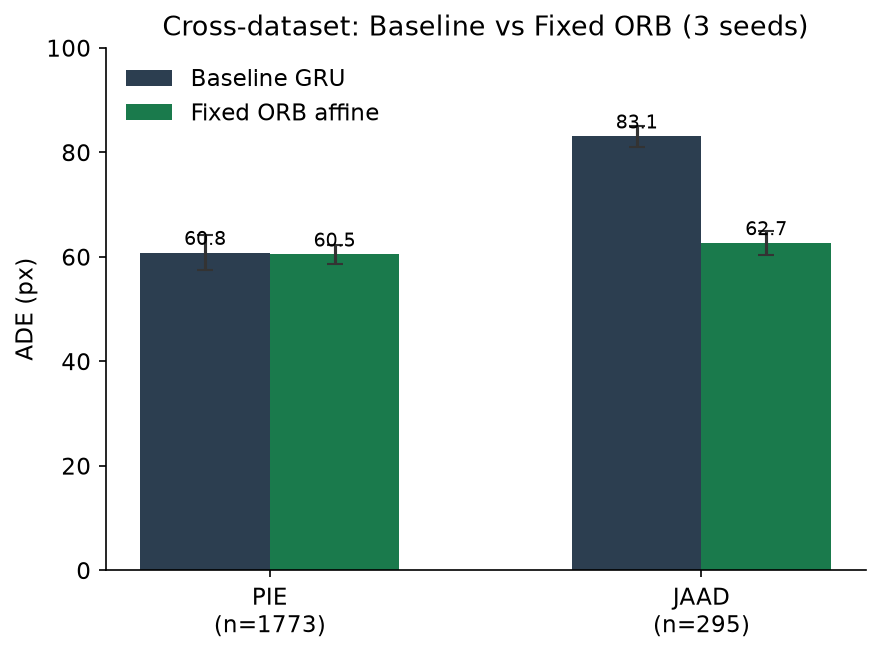
\includegraphics[width=\linewidth,height=0.20\textheight,keepaspectratio]{cross_dataset_ade.png}
    \caption{Cross-dataset ADE}
  \end{subfigure}\hfill
  \begin{subfigure}[t]{0.33\linewidth}
    \centering
    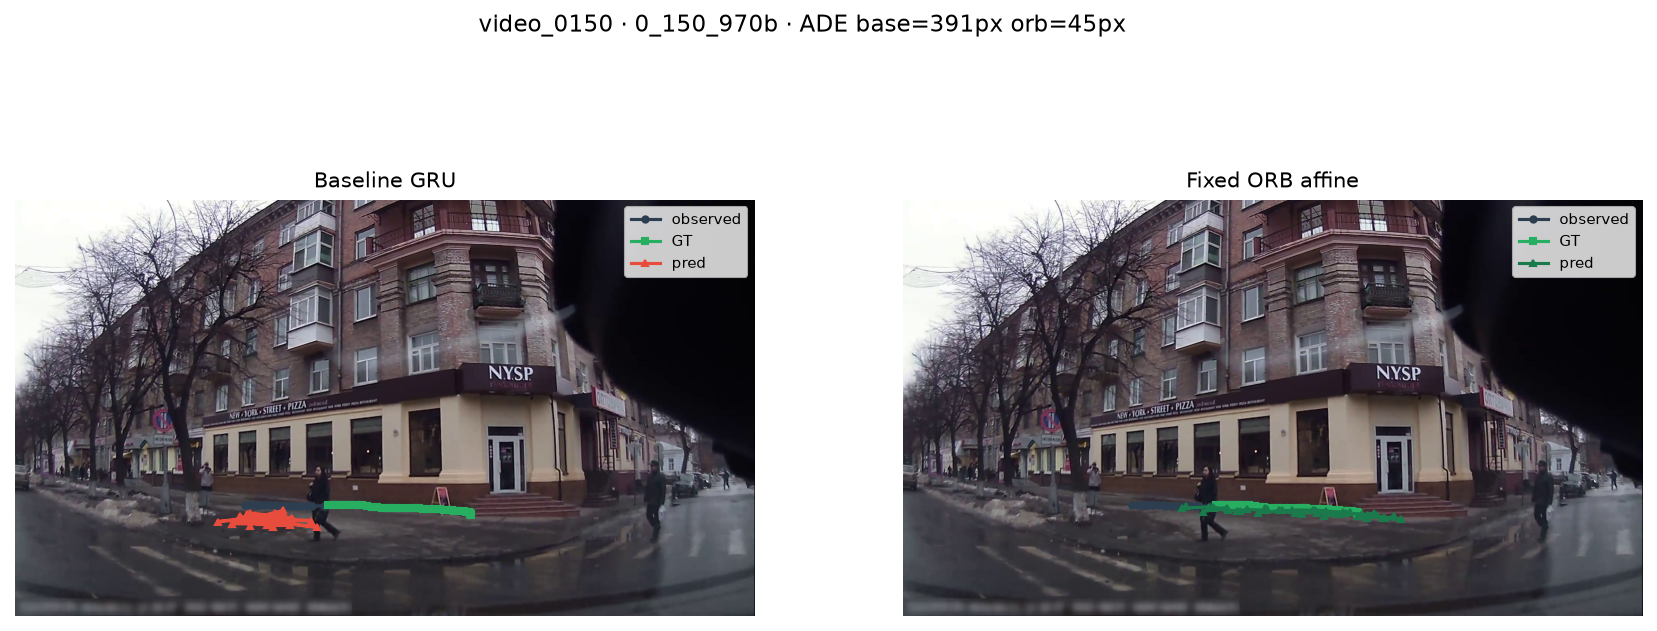
\includegraphics[width=\linewidth,height=0.20\textheight,keepaspectratio]{jaad_compare_0.png}
    \caption{Video 0150: 391$\rightarrow$45\,px}
  \end{subfigure}\hfill
  \begin{subfigure}[t]{0.33\linewidth}
    \centering
    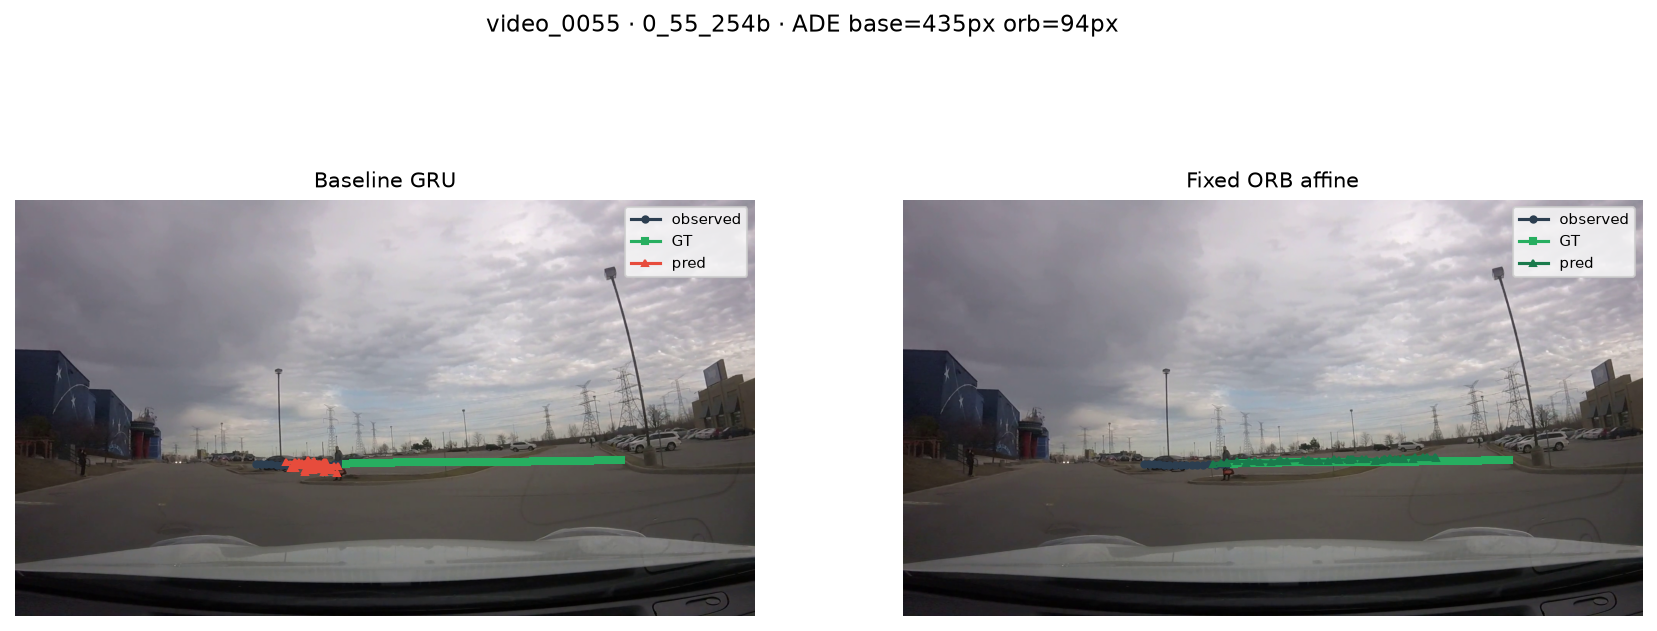
\includegraphics[width=\linewidth,height=0.20\textheight,keepaspectratio]{jaad_compare_1.png}
    \caption{Video 0055: 435$\rightarrow$94\,px}
  \end{subfigure}
  \caption{JAAD: PIE-neutral, JAAD-improving. Representative windows where compensation collapses large baseline errors.}
\end{figure}

%----------------------------------------------------------------------
\section{Intent Shortcut and Qualitative Examples}
\label{sec:qual}
%----------------------------------------------------------------------

Intent AUC rises monotonically with ego-motion exposure: fixed ORB (0.80) $<$ uncompensated baseline (0.89) $<$ GT speed (0.93).
Each increment injects ego-motion-correlated cues that can inflate apparent intent accuracy.

\begin{figure}[H]
  \centering
  \begin{subfigure}[t]{0.24\linewidth}
    \centering
    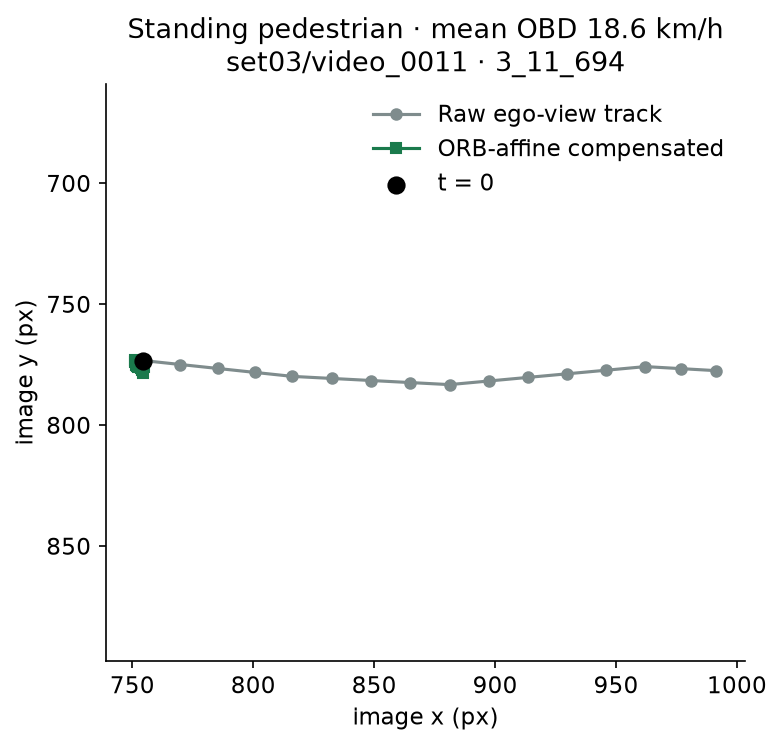
\includegraphics[width=\linewidth,height=0.19\textheight,keepaspectratio]{fig1_teaser.png}
    \caption{Standing pedestrian (18.6\,km/h)}
  \end{subfigure}\hfill
  \begin{subfigure}[t]{0.24\linewidth}
    \centering
    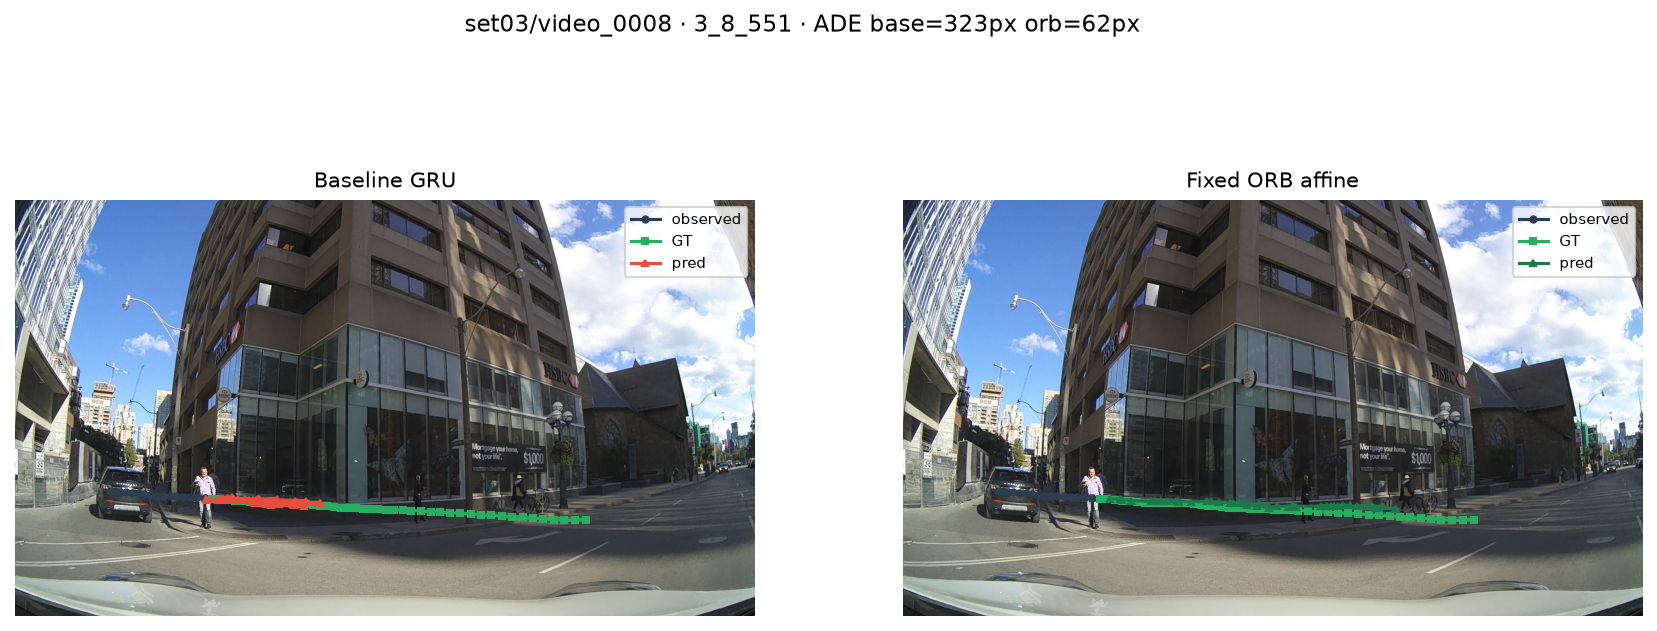
\includegraphics[width=\linewidth,height=0.19\textheight,keepaspectratio]{pie_compare_0.png}
    \caption{PIE trajectory overlay}
  \end{subfigure}\hfill
  \begin{subfigure}[t]{0.24\linewidth}
    \centering
    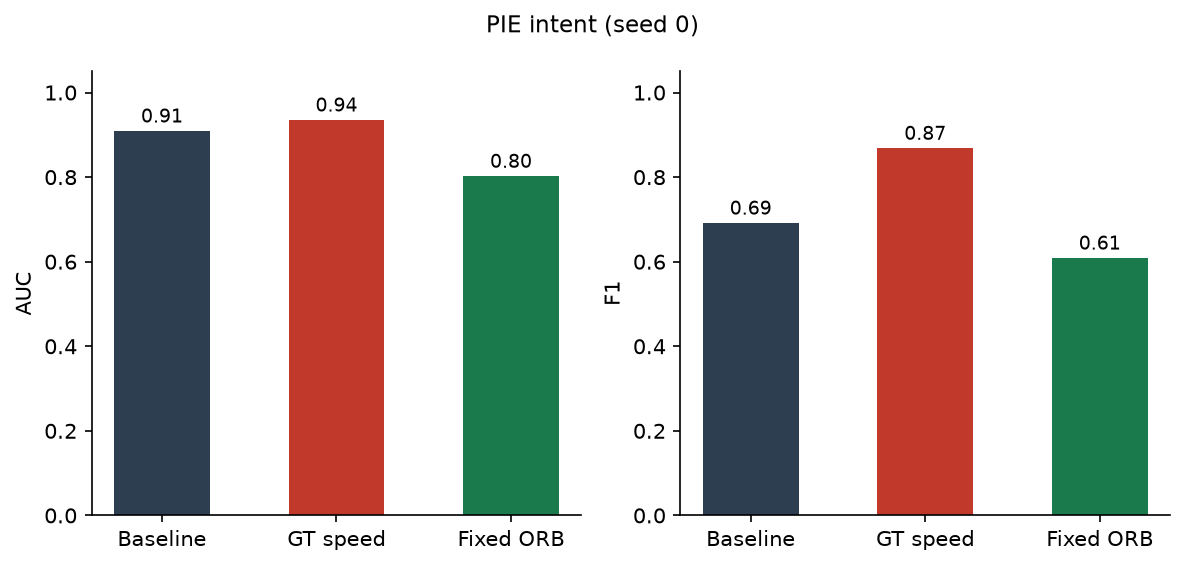
\includegraphics[width=\linewidth,height=0.19\textheight,keepaspectratio]{pie_intent_auc_f1.png}
    \caption{Intent AUC / F1}
  \end{subfigure}\hfill
  \begin{subfigure}[t]{0.24\linewidth}
    \centering
    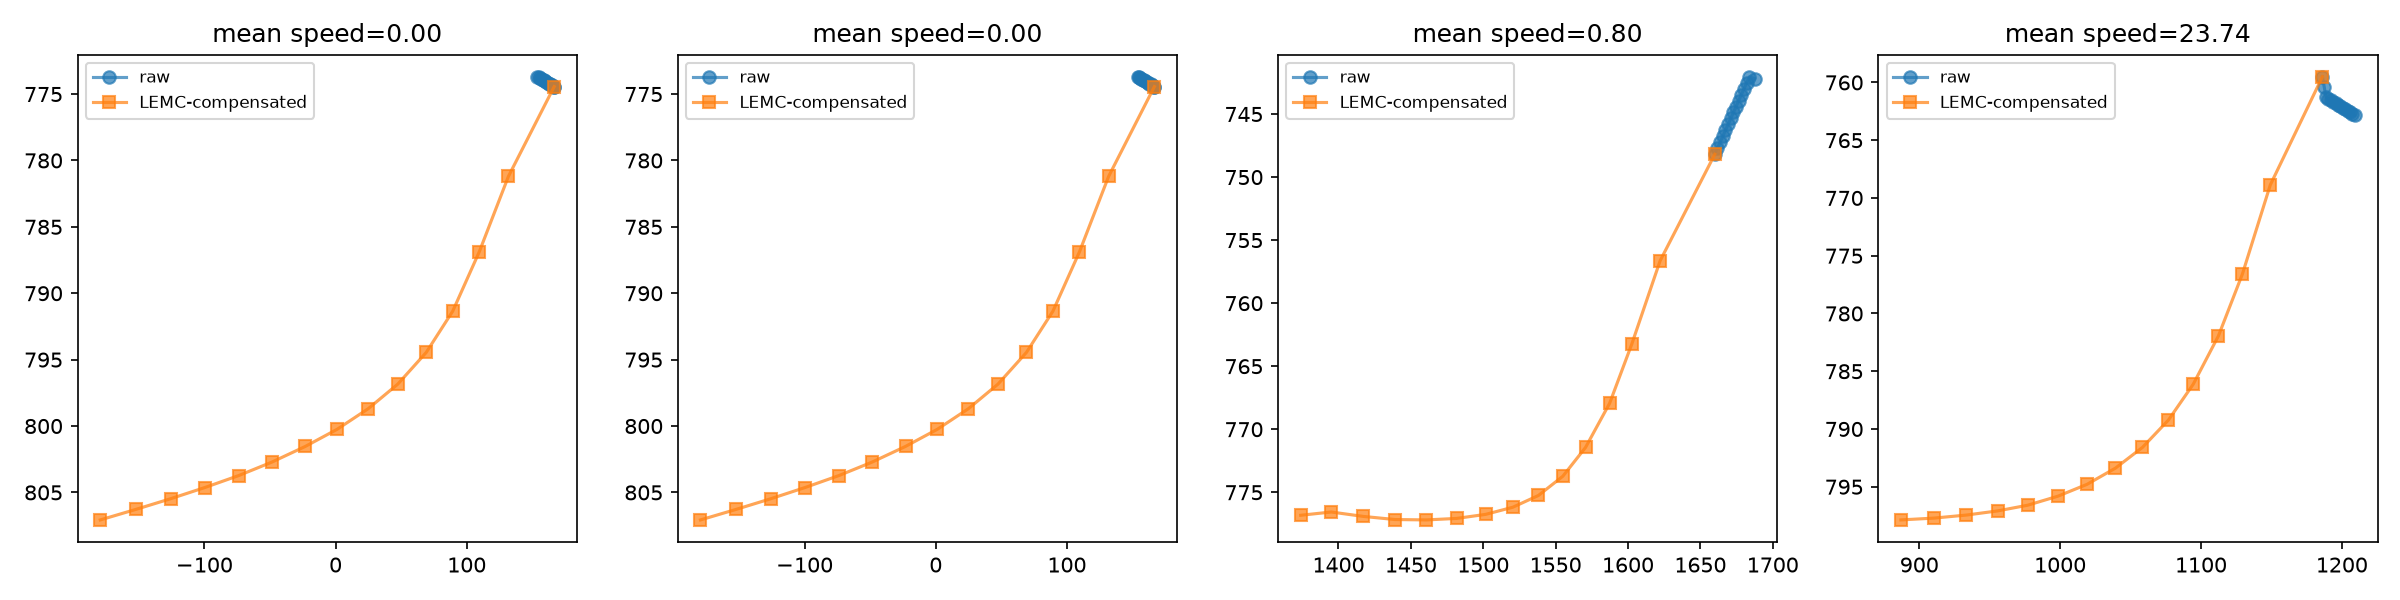
\includegraphics[width=\linewidth,height=0.19\textheight,keepaspectratio]{lemc_qualitative_pie_lemc_augmented_auxobd_seed0_test.png}
    \caption{LEMC failure (loops)}
  \end{subfigure}
  \caption{Qualitative summary. (a)~ORB flattens a standing pedestrian track; (b)~PIE overlay on real frame; (c)~intent vs.\ ego-motion; (d)~OBD-supervised LEMC loops instead of flattening.}
\end{figure}

%----------------------------------------------------------------------
\section{Takeaways}
%----------------------------------------------------------------------

\begin{enumerate}[leftmargin=1.5em,itemsep=4pt]
  \item \textbf{Physical gate before ADE.} Correlation with OBD ($R^2{=}0.30$) does not imply valid compensation; the variance gate separates the two.
  \item \textbf{Fixed beats learned.} Position-dependent full-affine ORB passes the gate and matches or beats baseline ADE; learned multi-agent residuals do not.
  \item \textbf{Dataset-dependent downstream gain.} PIE is trajectory-neutral ($-$0.5\,px); JAAD gains 20\,px because raw tracks carry more uncompensated ego drift without OBD.
  \item \textbf{Intent remains entangled.} Sensor-free geometry helps trajectory; intent metrics still track available ego-motion unless explicitly controlled.
\end{enumerate}

%----------------------------------------------------------------------
\appendix
\section{Figure file index}
%----------------------------------------------------------------------

\begin{table}[H]
  \centering
  \footnotesize
  \setlength{\tabcolsep}{4pt}
  \begin{tabular}{@{}p{0.42\linewidth}p{0.18\linewidth}p{0.30\linewidth}@{}}
    \toprule
    File (\texttt{paper/figures/}) & Gallery section & Role in \texttt{main.tex} \\
    \midrule
    \texttt{fig2\_architecture.png} & \S\ref{sec:method} & Method pipeline \\
    \texttt{fig\_main\_grid\_ade.png} & \S\ref{sec:pie} & PIE ADE bar chart \\
    \texttt{fig\_sign\_gate.png} & \S\ref{sec:pie} & Variance gate bars \\
    \texttt{lemc\_obd\_scatter\_...png} & \S\ref{sec:pie} & LEMC--OBD scatter \\
    \texttt{fig4\_orb\_obd\_scatter.png} & \S\ref{sec:orb} & ORB--OBD validation \\
    \texttt{fig5\_stratified\_ade.png} & \S\ref{sec:orb} & Stratified ADE \\
    \texttt{cross\_dataset\_ade.png} & \S\ref{sec:jaad} & PIE vs.\ JAAD bars \\
    \texttt{jaad\_compare\_0.png} & \S\ref{sec:jaad} & JAAD qualitative \\
    \texttt{jaad\_compare\_1.png} & \S\ref{sec:jaad} & JAAD qualitative \\
    \texttt{fig1\_teaser.png} & \S\ref{sec:qual} & Standing pedestrian \\
    \texttt{pie\_compare\_0.png} & \S\ref{sec:qual} & Frame overlay \\
    \texttt{pie\_intent\_auc\_f1.png} & \S\ref{sec:qual} & Intent AUC/F1 \\
    \texttt{lemc\_qualitative\_...png} & \S\ref{sec:qual} & LEMC failure case \\
    \bottomrule
  \end{tabular}
  \caption{All 13 PNG files used in the conference paper. \texttt{fig3\_qualitative.png} is not included (superseded).}
\end{table}

\vfill
\noindent\small\textit{Compile:} \texttt{cd paper \&\& pdflatex figures\_gallery.tex}

\end{document}
